\documentclass{beamer}

% Theme and Color Choices (feel free to change)
%\usetheme{Madrid} % A clean and professional theme
\usetheme {default}
\usecolortheme{beaver} % A pleasant color scheme
\setbeamercovered{transparent} % Fades out unrevealed items rather than hiding them

% Packages
\usepackage{amsmath} % For advanced math environments
\usepackage{amsfonts} % For mathematical symbols
\usepackage{amssymb} % For more symbols

\usepackage[dvipsnames]{xcolor}
\usepackage{tikz}
\usetikzlibrary{calc,shapes.geometric}

% Document Information
\title{Chromatic Contextuality}
\author{Karl Svozil, ITP, TU Wien, Vienna Austria}
\date{QIP25, V\"axj\"o, Sweden, 2025-06-10}

\begin{document}

% Title Page
\frame{\titlepage}

% Section 1: Introduction to Shannon Entropy
\section{Understanding Information}
\begin{frame}{Shannon Entropy: Quantifying Information}
    \begin{itemize}
        \item Shannon Entropy ($H$) measures the \alert{average uncertainty} or \alert{information content} of a random variable.
        \item The more uncertain an outcome (i.e., the more equally likely the possibilities), the higher its entropy, and thus, the more information we gain when observing it.
        \item It's typically measured in \alert{bits} (when using $\log_2$).
    \end{itemize}
    \pause
    \begin{block}{Formula for Shannon Entropy}
        For a discrete random variable $X$ with possible outcomes $x_1, x_2, \ldots, x_n$ and probabilities $P(x_1), P(x_2), \ldots, P(x_n)$:
        \begin{equation*}
            H(X) = -\sum_{i=1}^{n} P(x_i) \log_2 P(x_i) \quad \text{bits}
        \end{equation*}
    \end{block}
    \pause
    \begin{itemize}
        \item \alert{Assumption:} For these examples, we assume the initial underlying states are \textbf{equiprobable}.
    \end{itemize}
\end{frame}

% Section 2: 3-State System
\section{3-State System Analysis}
\begin{frame}{3-State System: Full Resolution}
    \begin{itemize}
        \item \textbf{System:} A system with 3 distinct states.
        \item \textbf{Observed Outcomes:} $\{0, 1, 2\}$
        \item \textbf{Probabilities (Equiprobable):}
            \begin{align*}
                P(0) &=
                P(1) =
                P(2) = 1/3
            \end{align*}
    \end{itemize}
    \pause
    \begin{block}{Calculating Information ($H_{full}$)}
        \begin{align*}
            H_{full} &= - \left[ \frac{1}{3} \log_2 \left(\frac{1}{3}\right) + \frac{1}{3} \log_2 \left(\frac{1}{3}\right) + \frac{1}{3} \log_2 \left(\frac{1}{3}\right) \right] \\
            &= -3 \times \frac{1}{3} \log_2 \left(\frac{1}{3}\right)
             = -\log_2 \left(\frac{1}{3}\right)
            = \log_2 3
        \end{align*}
        \begin{center}
            $\boldsymbol{H_{full} \approx 1.585 \text{ bits}}$
        \end{center}
    \end{block}
\end{frame}

\begin{frame}{3-State System: Collapsed Resolution}
    \begin{itemize}
        \item \textbf{Original States:} $\{0, 1, 2\}$ (equiprobable)
        \item \textbf{Mapping (Collapse):}
             $0 \rightarrow 0_{obs}$,  $1 \rightarrow 1_{obs}$ and  $2 \rightarrow 1_{obs}$
        \item \textbf{New Observed Outcomes:} $\{0_{obs}, 1_{obs}\}$
        \item \textbf{New Probabilities:}
            \begin{align*}
                P(0_{obs}) &= P(0) = 1/3 \\
                P(1_{obs}) &= P(1) + P(2) = 1/3 + 1/3 = 2/3
            \end{align*}
    \end{itemize}
    \pause
    \begin{block}{Calculating Information ($H_{collapsed}$)}
        \begin{align*}
            H_{collapsed} &= - \left[ P(0_{obs}) \log_2 P(0_{obs}) + P(1_{obs}) \log_2 P(1_{obs}) \right] \\
            &= - \left[ \frac{1}{3} \log_2 \left(\frac{1}{3}\right) + \frac{2}{3} \log_2 \left(\frac{2}{3}\right) \right]
            \approx 0.9183
        \end{align*}
        \begin{center}
            $\boldsymbol{H_{collapsed} \approx 0.918 \text{ bits}}$
        \end{center}
    \end{block}
\end{frame}

\begin{frame}{3-State System: Summary}
    \begin{itemize}
        \item \textbf{Full Resolution:} $H_{full} \approx \alert{1.585 \text{ bits}}$
        \item \textbf{Collapsed Resolution:} $H_{collapsed} \approx \alert{0.918 \text{ bits}}$
    \end{itemize}
    \pause
    \begin{block}{Information Loss}
        \begin{itemize}
            \item The act of collapsing states (losing the ability to distinguish between original 1 and 2) reduces the information obtained.
            \item Information Loss $= H_{full} - H_{collapsed} = 1.585 - 0.918 = \mathbf{0.667 \text{ bits}}$
        \end{itemize}
    \end{block}
\end{frame}

% Section 3: 4-State System
\section{4-State System Analysis}
\begin{frame}{4-State System: Full Resolution}
    \begin{itemize}
        \item \textbf{System:} A system with 4 distinct states.
        \item \textbf{Observed Outcomes:} $\{0, 1, 2, 3\}$
        \item \textbf{Probabilities (Equiprobable):}
            \begin{align*}
                P(0) &=
                P(1) =
                P(3) = 1/4
            \end{align*}
    \end{itemize}
    \pause
    \begin{block}{Calculating Information ($H_{full}$)}
        \begin{align*}
            H_{full} &= - \left[ \frac{1}{4} \log_2 \left(\frac{1}{4}\right) + \frac{1}{4} \log_2 \left(\frac{1}{4}\right) + \frac{1}{4} \log_2 \left(\frac{1}{4}\right) + \frac{1}{4} \log_2 \left(\frac{1}{4}\right) \right] \\
            &= -4 \times \frac{1}{4} \log_2 \left(\frac{1}{4}\right)
             = -\log_2 \left(\frac{1}{4}\right) = -(-2)
        \end{align*}
        \begin{center}
            $\boldsymbol{H_{full} = 2 \text{ bits}}$
        \end{center}
        \vspace{0.5em}
        \alert{A 4-state equiprobable system inherently provides 2 bits of information.}
    \end{block}
\end{frame}

\begin{frame}{4-State System: Collapsed Case}
    \begin{itemize}
        \item \textbf{Original States:} $\{0, 1, 2, 3\}$ (equiprobable)
        \item \textbf{Mapping (Collapse):}
             $\{0, 1\} \rightarrow 0'_{obs}$,
             $\{2, 3\} \rightarrow 1'_{obs}$
        \item \textbf{New Observed Outcomes:} $\{0'_{obs}, 1'_{obs}\}$
        \item \textbf{New Probabilities:}
            \begin{align*}
                P(0'_{obs}) &= P(0) + P(1) = 1/4 + 1/4 = 2/4 = 1/2 \\
                P(1'_{obs}) &= P(2) + P(3) = 1/4 + 1/4 = 2/4 = 1/2
            \end{align*}
    \end{itemize}
    \pause
    %\begin{block}{Calculating Information ($H_{collapsed\_ii}$)}
        \begin{align*}
            H &= - \left[ P(0'_{obs}) \log_2 P(0'_{obs}) + P(1'_{obs}) \log_2 P(1'_{obs}) \right] \\
            &= - \left[ \frac{1}{2} \log_2 \left(\frac{1}{2}\right) + \frac{1}{2} \log_2 \left(\frac{1}{2}\right) \right]
             = - \left[ \frac{1}{2}(-1) + \frac{1}{2}(-1) \right] =1
        \end{align*}

            $\boldsymbol{H = 1 \text{ bit}}$
        ---
        \alert{This scenario behaves like a fair coin flip.}
    %\end{block}
\end{frame}

\begin{frame}{4-State System: More Collapsed Case}
    \begin{itemize}
        \item \textbf{Original States:} $\{0, 1, 2, 3\}$ (equiprobable)
        \item \textbf{Mapping (More Collapse):}
                 $\{0, 1, 2\} \rightarrow 0''_{obs}$,
                $3 \rightarrow 1''_{obs}$
        \item \textbf{New Observed Outcomes:} $\{0''_{obs}, 1''_{obs}\}$
        \item \textbf{New Probabilities:}
            \begin{align*}
                P(0''_{obs}) &= P(0) + P(1) + P(2) = 1/4 + 1/4 + 1/4 = 3/4 \\
                P(1''_{obs}) &= P(3) = 1/4
            \end{align*}
    \end{itemize}
    \pause
    \begin{block}{Calculating Information ($H$)}
        \begin{align*}
            H &= - \left[ P(0''_{obs}) \log_2 P(0''_{obs}) + P(1''_{obs}) \log_2 P(1''_{obs}) \right] \\
            &= - \left[ \frac{3}{4} \log_2 \left(\frac{3}{4}\right) + \frac{1}{4} \log_2 \left(\frac{1}{4}\right) \right]
             \approx 0.81125
        \end{align*}
        \begin{center}
            $\boldsymbol{H \approx 0.811 \text{ bits}}$
        \end{center}
    \end{block}
\end{frame}

\begin{frame}{4-State System: Summary}
    \begin{itemize}
        \item \textbf{Full Resolution:} $H_{full} = \alert{2 \text{ bits}}$
        \item \textbf{Collapsed Case (ii):} $H_{collapsed\_ii} = \alert{1 \text{ bit}}$
        \item \textbf{More Collapsed Case (iii):} $H_{collapsed\_iii} \approx \alert{0.811 \text{ bits}}$
    \end{itemize}
    \pause
    \begin{block}{Observation}
        \begin{itemize}
            \item Each step of collapsing states leads to a \alert{reduction} in the measurable information content (entropy).
            \item The more states are merged, and the more skewed the resulting probabilities become, the lower the entropy.
        \end{itemize}
    \end{block}
\end{frame}

% Conclusion
\section{Conclusion}
\begin{frame}{Key Takeaway}
    \begin{itemize}
        \item The amount of information obtained from a system is directly related to its \alert{uncertainty} or \alert{entropy}.
        \item \alert{Collapsing or grouping outcomes} reduces the resolution of our observation, leading to:
            \begin{itemize}
                \item A decrease in the system's entropy.
                \item A \alert{loss of information} about the original, finer-grained states.
            \end{itemize}
        \item This demonstrates how information is lost when we approximate or simplify a more complex system.
    \end{itemize}
\end{frame}

\section{2-valued state in quantum mechanics}
\begin{frame}{2-valued state in 3 dimensions - spectral composition in terms of 1- and $d-1$ dimensional subspaces}
    \begin{center}
     \resizebox{0.4\textwidth}{!}{
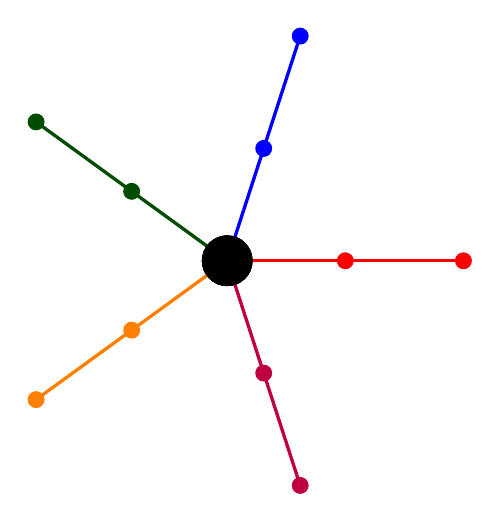
\begin{tikzpicture}
  % --- Definitions ---
  \def\centralRadius{0.3cm}
  \def\rayLength{3cm}
  \def\smallCircleRadius{0.1cm}
  \def\lineWidth{very thick}



  % --- Rays and Outer Circles ---
  % The variable for the color has been renamed to '\rayColor' to avoid
  % conflict with the built-in LaTeX '\color' command. This was the
  % source of the 'nullfont' error.
  \foreach \angle/\rayColor in {
    0/red,%
    72/blue,%
    144/Green!60!black,%
    216/orange,%
    288/purple%
  } {
    % Draw the ray using the explicit 'color=\rayColor' syntax for robustness.
    \draw[color=\rayColor, \lineWidth] (0,0) -- (\angle:\rayLength);

    % Draw the small circle at the midpoint of the ray.
    \filldraw[color=\rayColor] (\angle:{\rayLength/2}) circle (\smallCircleRadius);

    % Draw the small circle at the end of the ray.
    \filldraw[color=\rayColor] (\angle:\rayLength) circle (\smallCircleRadius);

    % --- Central Atom ---
    \filldraw[black, \lineWidth] (0,0) circle (\centralRadius);
  }

\end{tikzpicture}
}
    \end{center}
This is essentially a 3-state collapsed system: two states are mapped into 0 (painted in nonblack color), and one into 1 (painted black). In Hilbert space this represents a two-dimensional subspace, spanned by the eigenvectors of a continuum of orthonormal bases (here only 5 such bases are drawn).
\end{frame}

\section{Spectral Decomposition}
\begin{frame}{Spectral Decomposition of Maximal Versus Degenerate Operators}
Let $\{\mathbf{e}_i \vert 1 \le i \le d\}$ be an orthonormal basis.
\begin{itemize}
        \item \textbf{Maximal operator (von Neumann, 1931):}
Let  $\lambda_i$ be mutually distinct ``colors'', and
$\sum_{i=1}^d \lambda_i \vert \mathbf{e}_i \rangle \langle \mathbf{e}_i\vert$
        \item \textbf{Degenerate Operator:} let $1 \le j \le d$ be fixed, and
$\sum_{i=1}^d \delta_{ij} \vert \mathbf{e}_i \rangle \langle \mathbf{e}_i\vert$
    \end{itemize}
    \pause
\begin{block}{Postulate of Classicality}
Existence of classical d-ary elements of physical reality for certain finite quantum-inspired ``chromatic Kochen-Specker'' sets.
Again, chromatic noncontextuality is assumed: ``color is independent of the (hyper)edge''.
\end{block}
\end{frame}

\section{Some Results on Chromatic contextuality}
\begin{frame}{Some Results on Chromatic contextuality}

\begin{itemize}
        \item Whenever a ($d$-uniform hyper)graph has chromatic number $d$ it has at least $d$ two-valued states (by aggregation/contraction)
(M. H. Shekarriz and KS, JMP 63 (3), 032104 (2022) DOI: 10.1063/5.0062801).
        \item The Yu and Oh 3-uniform (hyper)graph has clique (element per hyperedge)number 3 but chromatic number 4 (and yet its set representable; same for Greechies $G_{32}$).
``Chromatic  Kochen Specker theorem'' (KS, Entropy 27(4), 387 (2025) DOI: 10.3390/e27040387).
        \item The house/pentagon/pentagram $d$-uniform hypergraph has one ``exotic'' 2-valued state that cannot be obtained from aggregation/contracting one of its 5 nonequivalent (modulo permuttations) colorings
 (KS, Entropy 27(4), 387 (2025) DOI: 10.3390/e27040387).
    \end{itemize}
\end{frame}

\section{Summary}
\begin{frame}{Summary}

\alert{Colorings might be a formidable tool to investigate quantum contextuality and classical probabilities.}
\end{frame}

\end{document}
